\documentclass{projetofinal-dcc}
%%%%%%%%%%%%%%%%%%%%%%%%%%%%%%%%%%%%%%%%%%%%%%%%%%%%%%%%%%%%
%P A C O T E S
%%%%%%%%%%%%%%%%%%%%%%%%%%%%%%%%%%%%%%%%%%%%%%%%%%%%%%%%%%%%
% Adicione aqui seus pacotes

%%%%%%%%%%%%%%%%%%%%%%%%%%%%%%%%%%%%%%%%%%%%%%%%%%%%%%%%%%%%
%I N I C I O  D O  D O C U M E N T O
%%%%%%%%%%%%%%%%%%%%%%%%%%%%%%%%%%%%%%%%%%%%%%%%%%%%%%%%%%%%
\begin{document}

% título da tese é obrigatório
\title{Título}

% autor é obrigatório; máximo de 3 autores
\author{Filipe Xavier Trindade dos Santos }{[Aqui entram os agradecimentos]}
\author{Lucas Simões de Souza Arnaud }{[Aqui entram os agradecimentos]}
\author{Thales Teixeira Pires}{[Aqui entram os agradecimentos]}

% orientador é obrigatório
\advisor[Profª.]{Silvana Rosseto,~Ph.D.}{}

% co-orientador é opcional
%\coadvisor[Prof.]{Nome do co-orientador,~M.Sc.}{}

% máximo de 3 integrantes da banca (orientador e co-orientador já são adicionados automaticamente)
\banca[Prof.]{Nome do participante banca 1,~D.Sc.}{COPPE~-~UFRJ}
\banca[Prof.]{Nome do participante banca 2,~Ph.D.}{COPPE~-~UFRJ}
%\banca[Prof.]{Nome do participante banca 3,~Ph.D.}{COPPE~-~UFRJ}

\location{Rio~de~Janeiro}{RJ}{Brasil}

% mês e ano de defesa
\date{Março}{2016}
\maketitle

\startdocument
%%%%%%%%%%%%%%%%%%%%%%%%%%%%%%%%%%%%%%%%%%%%%%%%%%%%%%%%%%%%
%A G R A D E C I M E N T O S
%%%%%%%%%%%%%%%%%%%%%%%%%%%%%%%%%%%%%%%%%%%%%%%%%%%%%%%%%%%% 
\makethankspage

%%%%%%%%%%%%%%%%%%%%%%%%%%%%%%%%%%%%%%%%%%%%%%%%%%%%%%%%%%%%
%R E S U M O
%%%%%%%%%%%%%%%%%%%%%%%%%%%%%%%%%%%%%%%%%%%%%%%%%%%%%%%%%%%%
\begin{abstract}{
  A eficiência de uma empresa está diretamente relacionada à forma como são conduzidos os seus processos internos. Quanto maior o tamanho da organização, mais importante se torna a sua capacidade de gestão para garantir que eles sejam executados com correção e dentro dos prazos esperados. Uma abordagem efetiva para atingir a eficiência organizacional é a automatização de processos de negócio.

O objetivo deste trabalho é apresentar duas diferentes tecnologias já existentes utilizadas para automatização de processos, o Redmine e os chamados BPMS, e suas principais características, e propor uma forma de integração entre elas, aproveitando as qualidades de ambas para oferecer maior qualidade de gestão, padronização e otimização de recursos na execução de processos de negócio.
}
\end{abstract}

%%%%%%%%%%%%%%%%%%%%%%%%%%%%%%%%%%%%%%%%%%%%%%%%%%%%%%%%%%%%
%A B S T R A C T
%%%%%%%%%%%%%%%%%%%%%%%%%%%%%%%%%%%%%%%%%%%%%%%%%%%%%%%%%%%%
\begin{englishabstract}{
  The efficiency of a company is directly related to the way its internal processes are conducted. The larger the size of the organization, the more important its management capacity becomes to ensure that they are executed with correctness and within the expected time frames. An effective approach to achieving organizational efficiency is the automation of business processes.

The objective of this work is to present two different technologies used for automation of processes, Redmine and the so-called BPMS, and their main characteristics, and to propose a way of integration between them, taking advantage of the qualities of both to offer higher management quality, standardization and optimization of resources in the execution of business processes.
}
\end{englishabstract}

%%%%%%%%%%%%%%%%%%%%%%%%%%%%%%%%%%%%%%%%%%%%%%%%%%%%%%%%%%%%
%L I S T A S
%%%%%%%%%%%%%%%%%%%%%%%%%%%%%%%%%%%%%%%%%%%%%%%%%%%%%%%%%%%%
% Figuras
\makefigurespage

% Tabelas
\maketablespage

% Algoritmos
\makelistingspage

% Abreviaturas (devem estar em ordem alfabética)
\makeabrevpage{\item [BPM] Business Process Management
\item [BPMS] Business Process Management System
\item [BPMI] Business Process Management Initiative
\item [BPMN] Business Process Management Notation
\item [XML] Extensible Markup Language
\item [OMG] Object Management Group


}

% Símbolos (devem estar em ordem alfabética)
\makesymbolspage{\input{elementos-pretextuais/simbolos}}

% Sumário 
\maketocpage

%%%%%%%%%%%%%%%%%%%%%%%%%%%%%%%%%%%%%%%%%%%%%%%%%%%%%%%%%%%%
%C O N T E Ú D O
%%%%%%%%%%%%%%%%%%%%%%%%%%%%%%%%%%%%%%%%%%%%%%%%%%%%%%%%%%%%
\startcontent
\chapter{Introdução}\label{chp:LABEL_CHP_1}

\section{Motivação}\label{sec:LABEL_CHP_1_SEC_A}
Os processos de negócio consistem numa sequência de atividades e serviços que  encadeados cumprem determinado objetivo ou função na organização em que é desempenhado. A automatização de processos de negócio consiste na aplicação de tecnologia, de forma que uma ou mais atividades de um processo possam ser automatizadas, reduzindo assim a dependência de atuação humana para sua execução.\footnote{\url{http://www.lipsum.com/}}.

\section{Objetivos}\label{sec:LABEL_CHP_1_SEC_B}
O objetivo geral deste trabalho é propor uma solução para automatização de processos complexos que também conta com interação humana, inclusive durante o fluxo destes. Vamos apresentar uma ferramenta que permite a modelagem de fluxos variados, facilita a configuração e implementação, bem como a utilização contínua por usuários com conhecimentos básicos de processo e o acompanhamento deste por um gerente.

\section{Organização do texto}\label{sec:LABEL_CHP_1_SEC_C}

\chapter{Conceitos básicos}\label{chp:LABEL_CHP_2}

\section{Introdução}\label{sec:LABEL_CHP_2_SEC_A}

\section{Processos}\label{sec:LABEL_CHP_2_SEC_B}
LUCAS VAI FAZER

\section{BPM}\label{sec:LABEL_CHP_2_SEC_C}
BPM é o acrônimo para o inglês Business Process Management, ou gestão de processos de negócio em português. Seu principal objetivo é oferecer uma abordagem sistemática para a execução, adaptação e melhoria de processos de negócio em um ambiente de constantes mudanças. O BPM pode ser encarado sob duas perspectivas distintas: o BPM como engenharia de software ou o BPM como disciplina de gestão.

\section{Activiti BPM}\label{sec:LABEL_CHP_2_SEC_D}


\section{Redmine}\label{sec:LABEL_CHP_2_SEC_E}
O Redmine é uma ferramenta de gerenciamento de projetos open-source. Foi criada por Jean-Philippe Lang em 2006. Desenvolvido em Ruby, utilizando a framework Rails, tem como objetivo dar flexibilidade de configuração ao usuário, e também ao desenvolvedor. A versão 3.1 deste software foi utilizada neste trabalho.


\chapter{Problema}\label{chp:LABEL_CHP_3}

\section{Introdução}\label{sec:LABEL_CHP_3_SEC_A}
LUCAS VAI FAZER

\section{Automatização de processos}\label{sec:LABEL_CHP_3_SEC_B}


\chapter{Redmine}\label{chp:LABEL_CHP_3}

\section{Introdução}\label{sec:LABEL_CHP_3_SEC_A}
Neste capítulo vamos explicar como o Redmine, uma ferramenta de gerenciamento de projetos foi utilizada para gestão de processos, ilustrando com um exemplo. Vamos apresentar ainda, as capacidade extensiva desta ferramenta, através do desenvolvimento de plugins. Por último vamos abordar as limitações do Redmine, que nos motivaram a desenvolver algo novo para atingir nosso objetivo em automatização de processos.

\section{Gestão de processos com o Redmine}\label{sec:LABEL_CHP_3_SEC_B}


\section{Como automatizar um processo?}\label{sec:LABEL_CHP_3_SEC_C}

\section{Plugins}\label{sec:LABEL_CHP_3_SEC_D}
O Redmine foi desenvolvido de forma a ser extensível por meio de plugins. É possível modificar um funcionalidade da ferramenta, ou criar novas funcionalidades sem precisar alterar o código desta. Os plugins são desenvolvidos em Rails, a mesma linguagem de programação do Redmine. 

Para possibilitar extensões de funcionalidades que envolvem enxertar pedaços de código no meio de uma classe ou de uma tela, o Redmine disponibiliza hooks em diversas partes da ferramenta. São tags com um identificador da parte do código em que estão inseridas. E para utilizar este hook basta incluir um hook listener num plugin, e direcionar qual arquivo ou método um determinado hook vai disparar.

\section{Limitações}\label{sec:LABEL_CHP_3_SEC_E}


\chapter{Activiti BPM}\label{chp:LABEL_CHP_4}

\section{Introdução}\label{sec:LABEL_CHP_4_SEC_A}
Criado em 2010 por ex-integrantes do projeto jBPM, o Activiti BPM é um projeto de código aberto sob a licença Apache 2, que provê um motor BPM leve e completo sob a especificação BPMN 2.0. O Activiti é desenvolvido sob a linguagem de programação Java e é facilmente integrável com aplicações existentes por sua leveza e API amigável.

Neste capítulo vamos apresentar como o Activiti BPM pode ser utilizado na automatização de processos de negócio. Vamos apresentar ainda, a capacidade de modelagem de processos através da notação BPMN utilizada pelo Activiti. Por último vamos abordar as vantagens e limitações desta ferramenta frente às demais opções do mercado.

\section{BPMN}\label{sec:LABEL_CHP_4_SEC_B}
BPMN (Business Process Management Notation) foi criada para representar processos de negócio em forma de diagrama, através de uma notação padronizada e de fácil entendimento por diferentes profissionais, sejam desenvolvedores, analistas de negócio ou gestores. Foi criada inicialmente pelo BPMI (Business Process Management Initiative) em 2004, mas atualmente é mantida e atualizada pela OMG (Object Management Group). Sua versão mais atual é a BPMN 2.0, publicada em 2011.

Foi concebida sob a perspectiva de ajudar a cobrir a falta de entendimento entre diferentes departamentos e organizações a cerca de um determinado processo ou conjunto de processos, algo muito frequente no ambiente corporativo. Além disso, através de sua notação padronizada em XML (Extensible Markup Language), diferentes ferramentas podem fazer o uso de sua auto-descrição para orquestração de processos de negócio, sejam eles automatizáveis ou não.

A notação define quatro grupos distintos de objetos para permitir a diagramação de um fluxo de negócio. Os objetos são classificados em artefatos, agrupadores, conectores e objetos de fluxo. São utilizadas figuras geométricas, como retângulos e círculos, além de linhas pontilhadas e tracejadas, entre outros elementos para representar cada um dos objetos que constituem a notação.

1) http://searchcio.techtarget.com/definition/Business-Process-Modeling-Notation

2) http://blog.iprocess.com.br/2012/11/um-guia-para-iniciar-estudos-em-bpmn-i-atividades-e-sequencia

3) https://www.fluig.com/blog/entendendo-melhor-o-bpmn/

\begin{figure}
  \centering
  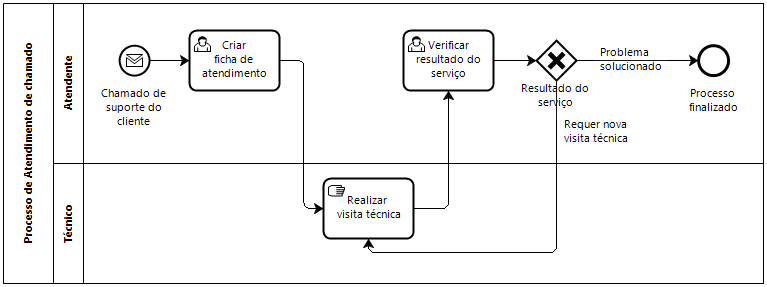
\includegraphics[width=1.0\textwidth]{imagens/bpmn_example.png}
  \caption{Exemplo de processo representado em BPMN}
  \label{fig:LABEL_FIG_1}
\end{figure}

\section{Gestão de processos com o Activiti BPM}\label{sec:LABEL_CHP_4_SEC_C}

\section{Como automatizar um processo?}\label{sec:LABEL_CHP_4_SEC_D}

\section{Vantagens e Limitações}\label{sec:LABEL_CHP_4_SEC_E}


\chapter{Integração Redmine e Activiti BPM}\label{chp:LABEL_CHP_5}

\section{Introdução}\label{sec:LABEL_CHP_5_SEC_A}
LUCAS VAI FAZER

\section{Implementação}\label{sec:LABEL_CHP_5_SEC_A}

\section{Resultados}\label{sec:LABEL_CHP_5_SEC_A}
\chapter{Lorem ipsum dolor sit amet}\label{chp:LABEL_CHP_2}

\section{Tables}\label{sec:LABEL_CHP_2_SEC_A}
Reference: \url{http://en.wikibooks.org/wiki/LaTeX/Tables}

\begin{table}[!h]
  \centering
  \begin{tabular}{ |l|l|l| }
    \hline
      Goalkeeper & Alan Smith & Paul Robinson \\
    \hline
      Lucus Radebe &  Mark Viduka & Michael Duberry \\
    \hline
      Eirik Bakke & Jamie McMaster & Jody Morris \\
    \hline
  \end{tabular}
  \caption{This table shows some data}
  \label{tab:LABEL_TAB_1}
\end{table}

\section{Images}\label{sec:LABEL_CHP_2_SEC_B}
Reference: \url{http://en.wikibooks.org/wiki/LaTeX/Importing_Graphics}

\begin{figure}
  \centering
%  \includegraphics[width=0.6\textwidth]{imagens/chick.png}
  \caption{Chick}
  \label{fig:LABEL_FIG_1}
\end{figure}

\section{Equations}\label{sec:LABEL_CHP_2_SEC_C}
Reference: \url{http://en.wikibooks.org/wiki/LaTeX/Mathematics}

Also: \url{http://en.wikibooks.org/wiki/LaTeX/Advanced_Mathematics}

\begin{equation}
  (x + y)^2 = x^2 + 2xy + y^2
  \label{eq:LABEL_EQ_1}
\end{equation}

\section{Listings}\label{sec:LABEL_CHP_2_SEC_D}
Reference: \url{http://en.wikibooks.org/wiki/LaTeX/Source_Code_Listings}

\codec{C}{alg:LABEL_CODE_1}{codigos/codigo-c.txt}

\codejava{Java}{alg:LABEL_CODE_2}{codigos/codigo-java.txt}

\section{References}\label{sec:LABEL_CHP_2_SEC_E}
\begin{itemize}
  \item Referencing \refchapter{chp:LABEL_CHP_1}
  \item Referencing \refsection{sec:LABEL_CHP_1_SEC_A}
  \item Referencing \refsection{sec:LABEL_CHP_1_SEC_C}
  \item Referencing \reftable{tab:LABEL_TAB_1}
  \item Referencing \reffigure{fig:LABEL_FIG_1}
  \item Referencing \refequation{eq:LABEL_EQ_1}
  \item Referencing \reflisting{alg:LABEL_CODE_1}
  \item Referencing \refappendix{chp:LABEL_APP_1}
\end{itemize}
\pagebreak

%%%%%%%%%%%%%%%%%%%%%%%%%%%%%%%%%%%%%%%%%%%%%%%%%%%%%%%%%%%%
% B I B L I O G R A F I A
%%%%%%%%%%%%%%%%%%%%%%%%%%%%%%%%%%%%%%%%%%%%%%%%%%%%%%%%%%%%
% Retirar esta parte se o trabalho não tiver bibliografia
\makebibspage{abnt}{elementos-postextuais/referencias}

%%%%%%%%%%%%%%%%%%%%%%%%%%%%%%%%%%%%%%%%%%%%%%%%%%%%%%%%%%%%
% A P E N D I C E
%%%%%%%%%%%%%%%%%%%%%%%%%%%%%%%%%%%%%%%%%%%%%%%%%%%%%%%%%%%%
% Retirar esta parte se o trabalho não tiver anexos
\appendix
\chapter{Processo de Precificação em BPMN}\label{chp:LABEL_APP_1}

    \lstset{
    language=xml,
    tabsize=3,
    %frame=lines,
    caption=Código do Processo de Precificação em BPMN,
    label=code:process_bpmn,
    frame=shadowbox,
    rulesepcolor=\color{gray},
    xleftmargin=20pt,
    framexleftmargin=15pt,
    keywordstyle=\color{blue}\bf,
    commentstyle=\color{OliveGreen},
    stringstyle=\color{red},
    numbers=left,
    numberstyle=\tiny,
    numbersep=5pt,
    breaklines=true,
    showstringspaces=false,
    basicstyle=\footnotesize,
    emphstyle={\color{magenta}}}
    \lstinputlisting{codigos/process.xml}

\chapter{REST de Definições de Tarefas}\label{chp:LABEL_APP_1}

     \lstset{
    language=java,
    tabsize=3,
    %frame=lines,
    caption=REST de Definições de Tarefas,
    label=code:task_definition_service,
    frame=shadowbox,
    rulesepcolor=\color{gray},
    xleftmargin=20pt,
    framexleftmargin=15pt,
    keywordstyle=\color{blue}\bf,
    commentstyle=\color{OliveGreen},
    stringstyle=\color{red},
    numbers=left,
    numberstyle=\tiny,
    numbersep=5pt,
    breaklines=true,
    showstringspaces=false,
    basicstyle=\footnotesize,
    emphstyle={\color{magenta}}}
    \lstinputlisting{codigos/TaskDefinitionService.java}

\end{document}